\section{\textbf{Semi-supervised\\ Exploiting Unlabeled Data}}

%%%%%%%%%%%%%%%%%%%%%%%%%%%%%%%%%%%%%%%%%%%%%%%%%%%%%%%%%%%%%%%%%%%%%%%%%%%%%%%%
\subsection{\textbf{Labeling strategy}}

My approach to semi-supervised learning is to iteratively expand the labeled data and retrain the classifier.

\begin{algorithm}[]
  \caption{Semi-Supervised}
  \KwIn{$D_{u}$ as unlabeled data, $D_{l}$ as labeled data, $ratio$, $threshold$}
  \KwOut{Model parameters $\theta$}
  $\hat{D}_l \leftarrow D_l, \hat{D}_u \leftarrow D_u$\;
  \While{$\hat{D}_u > (1-ratio)*D_u$}
  {
    $\theta \leftarrow \text{Train}(\hat{D}_l)$\;
    $D'_u \leftarrow \text{Predict}(\theta, \hat{D}_u)$\;
    $\hat{D}_l \leftarrow \text{Expand}(\hat{D}_l, D'_u, threshold)$\;
    $\hat{D}_u \leftarrow \text{Remove}(D'_u, threshold)$\;
  }
  return $\theta$\;
\end{algorithm}

The first thing is to decide which labels to include in $\hat{D}_l$ in every iteration. We choose to include the most confident predictions (i.e., the probability of these predictions should be bigger than the $threshold$).

The second thing is to decide the stopping criterion. Instead of choosing a fixed number of iterations, we choose to stop when a certain $ratio$ of $D_u$ has been added into the labeled training data $\hat{D}_l$.

In order to make our performances better, We tried different combinations of $ratio$ and $threshold$.

\subsection{\textbf{Labeled Data Size Analysis}}

Usually, larger datasets can help us avoid over-fitting. If our model has many parameters and it isn't fed enough data, then it will tend to memorize the training set and perform poorly on the dev/test set. To avoid this phenomenon, except for using special training techniques like regularization, we can also use a semi-supervised method. By using semi-supervised learning, it is possible to combine the advantages of working with a smaller labeled dataset to guide the learning process and a larger unlabeled dataset to increase the generalizability of the solution. 

In order to make it possible for semi-supervised learning methods to make the most of the labeled and unlabeled data, some assumptions are needed for the underlying structure of data space. The labeled and unlabeled data points should share the same data space. If the distributions are hugely different for those two data, then adding labeled data may and confuse our model and thus decrease our performances.

\subsection{\textbf{Feature Analysis}}

There should exist an overlapping between the unlabeled data and labeled data. When adding those unlabeled data into our training data, we will augment the effect of those overlapped words. Whether using BoW or TF-IDF, the features of overlapped words will change enormously, which will further lead to the result that their weights may change significantly. Meanwhile, for those not overlapped words, while their features may remain the same, it can be regarded as their weights decreases.

If some words appear in the unlabeled data and then be further added into the training set. Then we can assume their initial weight is zero. After retraining on the new training data, they will have a weight. 

\subsection{\textbf{Performances}}

We can refer to figure~\ref{fig:threshold} to see the performances of $Ratio=0.7$ on different thresholds. Overall speaking, compared with supervised learning, the performances on development set is decreasing as we add more labeled data to our training sets. 

\begin{figure}[!ht]
    \centering
    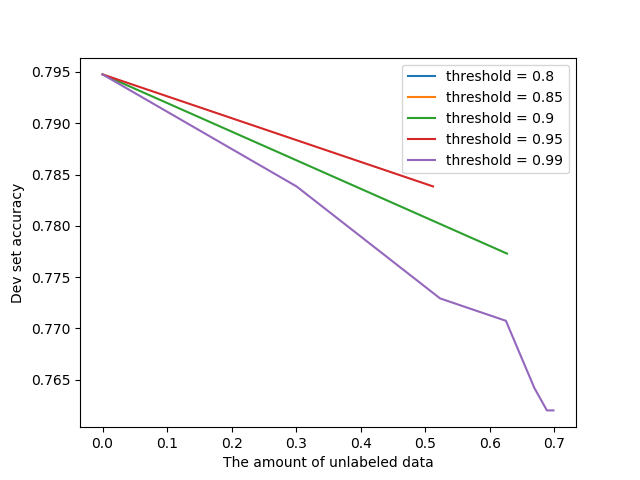
\includegraphics[width=0.45\textwidth]{files/figs/semi.png}
    \caption[]%
    {{\small Performances of Ratio=0.7 on different thresholds}}
    \label{fig:threshold}
\end{figure}

The first thing we should notice is our model can achieve a high accuracy of about 0.8 on the development set and  1.0 on the training set. Thus, our threshold should be bigger than 0.8.

What we should know is that the unlabeled data is so noisy and it even contains some Chinese and Japanese words. If not selected precisely, adding those data as labeled data may confuse your model and decrease the accuracy.

When the threshold is low, each iteration we will have more confident data and thus can add more labeled data into our training data. So after two or three iterations then we will achieve the stopping criterion since the amount of unlabeled data is larger than our ratio. However, a lower threshold means you are less confident about the precision of your prediction. As the threshold increases, each iteration will get a smaller amount of confident data. Thus, we will need more iterations. The higher threshold should mean the prediction is more accurate. There is a tradeoff between the precision and the number of iterations. 

\subsection{\textbf{Error Analysis}}

I sampled the following sentences and their respective labels generated by supervised learning and semi-supervised learning. 

\begin{itemize}
\item \textit{"This is a serious matter that needs to be addressed.. I've had my fair share of chipotle, and this one by far is the most stingiest.. Us Fat ass American's".} Supervised Model labeL: Negative. Semi-Supervised Model Label: Positive. Ground Truth: Negative.
\item \textit{'Went there for the first time last night to celebrate a friends birthday.  OMG!  The porkchops were unbelievable. Met the owner, Eddie.  Good friends, great food'} Supervised Model labeL: Negative. Semi-Supervised Model Label: Positive. Ground Truth: Positive.
\end{itemize}

\begin{table}[ht]  %table 里面也可以嵌套tabular,只有tabular是不能加标题的
\centering  %表格居中
\caption{Statistical Information}
\begin{tabular}{lccc}
\hline
&    \textbf{Train} & \textbf{Dev} & \textbf{Unlabeled} \\
\hline
 \textbf{Total} & 4582 & 458 & 91524 \\
 \textbf{Positive}   & 2291 &  229 &  -   \\
 \textbf{Negative} &  2291 &  229  &  -  \\
\hline
\end{tabular}
\label{tab:stat}
\end{table}

\begin{table}[ht]  %table 里面也可以嵌套tabular,只有tabular是不能加标题的
\centering  %表格居中
\caption{Labels for Unlabeled data}
\begin{tabular}{lcc}
\hline
&    \textbf{Supervised Model} & \textbf{Semi-Supervised Model}  \\
\hline
 \textbf{Total} & 91524 & 91524  \\
 \textbf{Positive}   & 44202 &  43325 \\
 \textbf{Negative} & 47322  &  48199  \\
\hline
\end{tabular}
\label{tab:unlabel}
\end{table}

We can see from Table~\ref{tab:stat} that the original dataset is pretty balanced. It contains the same number of positive samples and negative samples.

However, according to Table~\ref{tab:unlabel}, the distribution of our predicted label isn't like the original one. The semi-supervised model tends to predict more negative labels than the supervised model. There are 4331 different labels out of 91524 lines in the prediction from our two models.







